% !TEX root = main.tex

%%%%%%%%%%%%%%%%%%%%%%%%%%%%%%%%%%%%%%%%%%%%%%%%%%%%%%%%%%%%%%%%%%%%%%%%%%%%%%%%%%%%%%%%%%%%%%%%
\section{実験}
%%%%%%%%%%%%%%%%%%%%%%%%%%%%%%%%%%%%%%%%%%%%%%%%%%%%%%%%%%%%%%%%%%%%%%%%%%%%%%%%%%%%%%%%%%%%%%%%

\subsection{概要}
    本実験では図2の階段状の関数の代わりに,図3の回路を用いて,
    図4に示すような矩形波$(4\mathrm{~V}$\,peak-to-peak,duty比$1: 1$)
    を入力するものとする.時刻$t=0$で図2に示す$-V \rightarrow+V$の
    (昇りの)階段状の電圧を回路に印加し,次に,十分長い時間がたったあとの時刻
    $t=T / 2$で,図2と逆の$+V \rightarrow-V$の(下りの)階段状の
    電圧を印加する.このあと更に,時刻$t=T$で再び$-V \rightarrow+V$の
    (昇りの)階段状の電圧を回路に印加する.つまり,周期的な過渡現象を起こさせるわけで
    ある.ただし,(3)\sim(5)式の指数関数中の定数$\alpha-\beta$あるいは
    $\alpha$が適当に大きいこと,いいかえれば減哀に要する時間の目安である
    $1 /(\alpha-\beta)$あるいは$1 / \alpha$が矩形波の半周期$T / 2$より
    小さいことが必要である.
    
    なお,キャパシタの電荷の時間変化を観測するには,
    キャパシタCの両端の電圧変化をみればよく,電流の時間変化を観測するには,
    抵抗$\mathrm{R}$の両端の電圧変化をみればよい.また,電源の内部インピーダンス
    も考慮に入れて考察を行うこと.回路図では純抵抗と仮定し,$r_0$と表しており,
    実験に使用する発振器においては$r_0=600\,\Omega$とする.

\subsection{実験手順}    
    \begin{enumerate}
        \item 必要器具の点検後,ブレッドボード上の回路作成と機器の結線を行う.
        ブレッドボード内の線の接続,およひ機器のグラウンドレベルが正しく共通にとれている
        ことを確認する.また,オシロスコープの掃引トリガのタイミングとして,
        印加電圧の立ら上がりを取るようにオシロスコーブを調整する.

        \item  発振器の微調整つまみを調整して,出力電圧を$4 \mathrm{~V}$\,peak-to-peak
        にする.また,発振器の周波数を微調整して,横軸10目盛りでほぼ1周期分が表示される
        ように設定する.

        \item キャパシタCの両端の電圧が予測した過渡特性と一致することがオシロスコープの
        画面上で読めたら,指道教員またはTAの確認を受ける.もし,予測との間に顕著な差異が
        現れたら,その原因について考えること.

        \item 教員またはTAの確認が済んだら,波形をプリントアウトする.

        \item $R$および$L$の両端電圧についてはどうか.測定波形と予測波形とを比較・確認
        した上で,プリントアウトする.

        \item 指定された$L, C, R$の組み合わせについて,上記の手順を繰り返す.
    \end{enumerate}

\newpage

\subsection{実験条件}
使用する素子の条件は$\mathrm{L}=1\,\mathrm{mH}$,
$\mathrm{C}=4700\,\mathrm{pF},100\,\mathrm{pF}$,
$\mathrm{R}=1\,\mathrm{k}\Omega$である.

\subsection{使用機器}
\begin{enumerate}
    \item RC発信機(ケンウッド\quad AG-203A)
    \item DSO(Tektronix\quad TBS1022)
    \item ブレッドボード
    \item Qucs\quad 0.0.16
\end{enumerate}

\begin{figure}[H]
    \begin{center}
        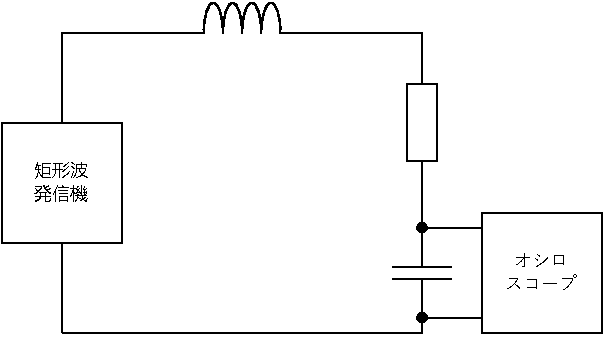
\includegraphics[]{figure2.drawio.pdf}
        \caption{測定回路}
    \end{center}
\end{figure}

\begin{figure}[H]
    \begin{center}
        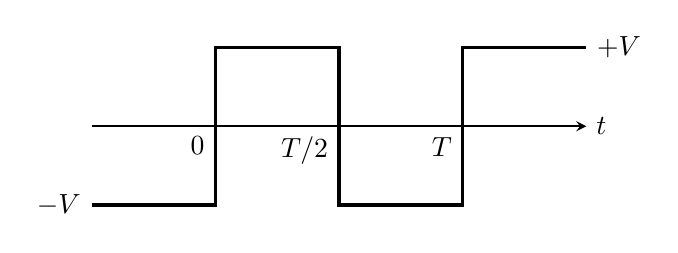
\begin{tikzpicture}
            \draw[->,>=stealth,semithick] (-pi,0)--(pi,0) node[right]{$t$}; %x軸
            \draw[very thick] (-pi,-1) node[left]{$-V$} -- (-pi/2,-1) -- (-pi/2,0) node[below left]{$0$} -- (-pi/2,1) -- (0,1) -- (0,0) node[below left]{$T/2$} -- (0,-1) -- (pi/2,-1) -- (pi/2,0) node[below left]{$T$}  -- (pi/2,1) -- (pi,1) node[right]{$+V$};
        \end{tikzpicture}
        \caption{矩形波}
    \end{center}
\end{figure}